\documentclass{standalone}
\usepackage{tikz}
\usepackage{ctex,siunitx}
\setCJKmainfont{Noto Serif CJK SC}
\usepackage{tkz-euclide}
\usepackage{amsmath}
\usetikzlibrary{patterns, calc}
\usetikzlibrary {decorations.pathmorphing, decorations.pathreplacing, decorations.shapes,}
\begin{document}
\small
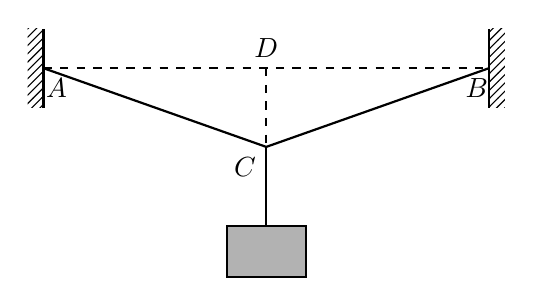
\begin{tikzpicture}[>=stealth, thick]
  \fill [pattern = north east lines] (-3.03,-.5) rectangle (-2.83,.5);
  \draw(-2.83,.5)--(-2.83,-.5);
  \fill [pattern = north east lines] (3.03,-.5) rectangle (2.83,.5);
  \draw(2.83,.5)--(2.83,-.5);
  \draw [dashed] (-2.83,0)  --node[above]{$D$} (2.83,0);
  \node at (-2.4,0) [below left]{$A$};
  \node at (2.4,0) [below right]{$B$};
  \draw [dashed] (0,0)  -- (0,-1.0)node[below left]{$C$};
  \draw  (0,-1.0)  -- (0,-2.0);
  \draw (-2.83,0)--(0,-1.0)--(2.83,0);
  \draw [fill=black!30] (-.5,-2.0) rectangle (.5,-2.65);
\end{tikzpicture}
\end{document}